\chapter{Hot Gas Layer Temperature and Depth}

CFAST simulated all of the chosen experiments.  Details of the comparisons with experimental data, are provided in Appendix B.  The results are organized by quantity as follows:

\begin{itemize}
\item hot gas layer (HGL) temperature and height
\item ceiling jet temperature
\item plume temperature
\item flame height
\item oxygen and carbon dioxide concentration
\item smoke concentration
\item compartment pressure
\item radiation heat flux, total heat flux, and target temperature
\item wall heat flux and surface temperature
\end{itemize}

The measure of model \emph{accuracy} used throughout this study is related to experimental uncertainty. Reference \cite{NRCNUREG1824}  discusses this issue in detail. In brief, the accuracy of a measurement, for example, a gas temperature, is related to the measurement device, a thermocouple. In addition, the accuracy of the model prediction of the gas temperature is related to the simplified physical description of the fire and the accuracy of the input parameters, especially the specified heat release rate. Ideally, the purpose of a validation study is to determine the accuracy of the model in the absence of any errors related to the measurement of both its inputs and outputs. Because it is impossible to eliminate experimental uncertainty, at the very least a combination of the uncertainty in the measurement of model inputs and output can be used as a yardstick. Dotted lines in figure \ref{fig:HGL_Temperature_Scatter}  show this combined uncertainty estimate for HGL temperature. Corresponding estimates are included for other quantities in later sections. If the numerical prediction falls within the range of uncertainty attributable to both the measurement of the input parameters and the output quantities, it is not possible to further quantify its accuracy. At this stage, it is said that the prediction is within experimental uncertainty.

Note that the calculation of relative difference is based on the temperature rise above ambient, and the layer depth, that is, the distance from the ceiling to where the hot gas layer descends.  Where the model over-predicts the HGL temperature or the depth of the HGL, the relative difference is a positive number. This convention is used throughout this report where the model over-predicts the severity of the fire, the relative difference is positive; where it under-predicts, the difference is negative.

Arguably the most frequent question asked about a fire is, ``How hot did it become''  Temperature in the upper layer of a compartment is an obvious indicator to answer this question.  Peak temperature, time to peak temperature, or time to reach a chosen temperature tenability limit are typical values of interest.  Quality of the prediction (or measurement) of layer interface position is more difficult to quantify.  Although observed in a range of experiments, the two-layer assumption is in many ways just a convenience for modeling.  In experimental measurements, temperature is typically measured with an array of thermocouples from floor to ceiling.  This floor to ceiling temperature profile can then used to estimate a hot gas layer height and the temperature of the upper and lower gas layers \cite{Janssens:1992} \cite{McGrattan:2003} consistent with the two-zone assumption. Appendix A provides details of the calculation.

From a standpoint of hazard, time of descent to a chosen level may be a reasonable criterion (assuming some in the room will then either be forced to crawl beneath the interface to breathe the ``clean'' atmosphere near the floor or be forced to breath the upper layer gases).  Minimum values may also be used to indicate general agreement.  For the single-room tests with furniture or wall-burning, these are appropriate indicators to judge the comparisons between model and experiment.  For the more-closely steady-state three- and four-room tests with corridor or the multiple-story building tests, a steady-state average may better characterizes the nature of the experiment.

A good prediction of the HGL height is largely a consequence of a good prediction of its temperature because smoke and heat are largely transported together and most numerical models describe the transport of both with the same type of algorithm.  Typically, CFAST slightly over-predicts the HGL temperature, most often within experimental uncertainty.  Hot gas layer height is typically within experimental uncertainty for well-ventilated tests and near floor level for under-ventilated tests where compartments are closed to the outside.  For HGL height, both open- and closed-door tests are included.  For closed-door tests, visual observations typically show that the HGL fills the entire compartment volume from floor to ceiling, inconsistent with the calculated results for the experimental data.  Thus, the comparisons with experimental values of HGL height for closed-door tests are expected to have larger differences that those for open-door tests.

Figures \ref{fig:HGL_Temperature_Scatter} and \ref{fig:HGL_Height_Scatter} shows a comparison of predicted and measured values for HGL temperature and depth. Appendix B provides individual graphs of model and experimental values.


\section{Summary of Hot Gas Layer Temperature and Height}
\label{HGL Temperature}
\label{HGL Temperature: Natural Ventilation}
\label{HGL Temperature: Forced Ventilation}
\label{HGL Temperature: No Ventilation}
\label{HGL Depth}
\label{HGL Depth: Closed Compartments}
\label{HGL Depth: Open Compartments}

\begin{figure}
\begin{tabular*}{\textwidth}{l@{\extracolsep{\fill}}r}
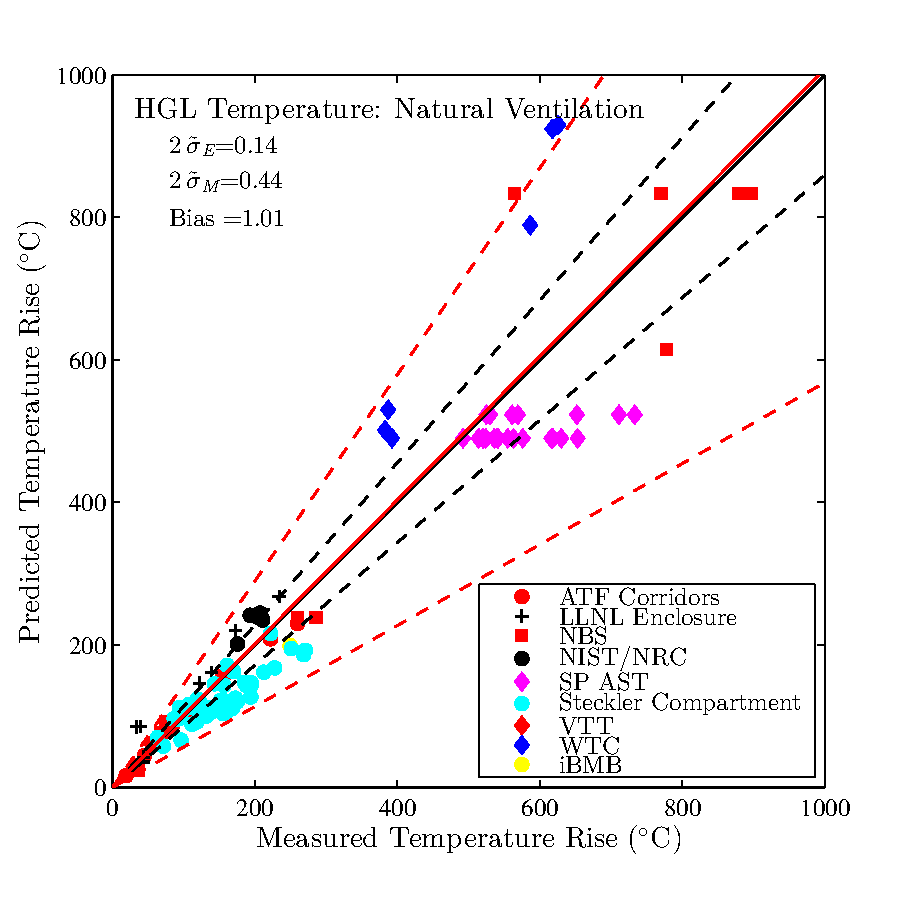
\includegraphics[width=3.0in]{FIGURES/ScatterPlots/HGL_Temperature_Natural_Ventilation} &
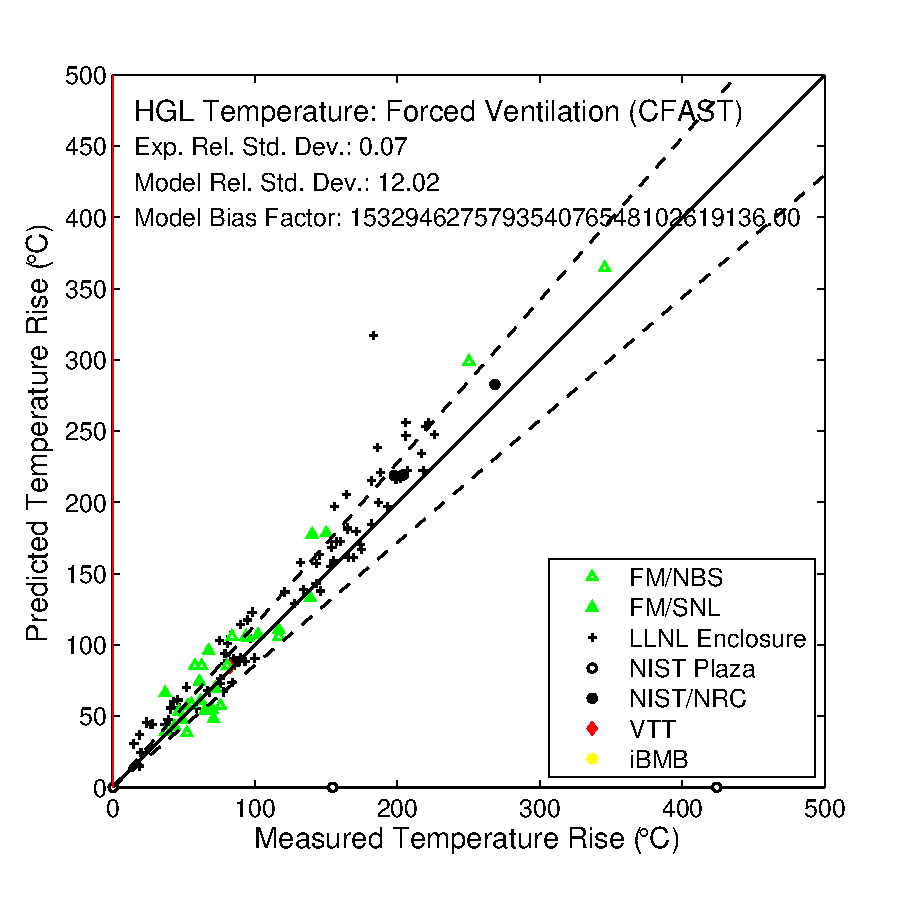
\includegraphics[width=3.0in]{FIGURES/ScatterPlots/HGL_Temperature_Forced_Ventilation} \\
\multicolumn{2}{c}{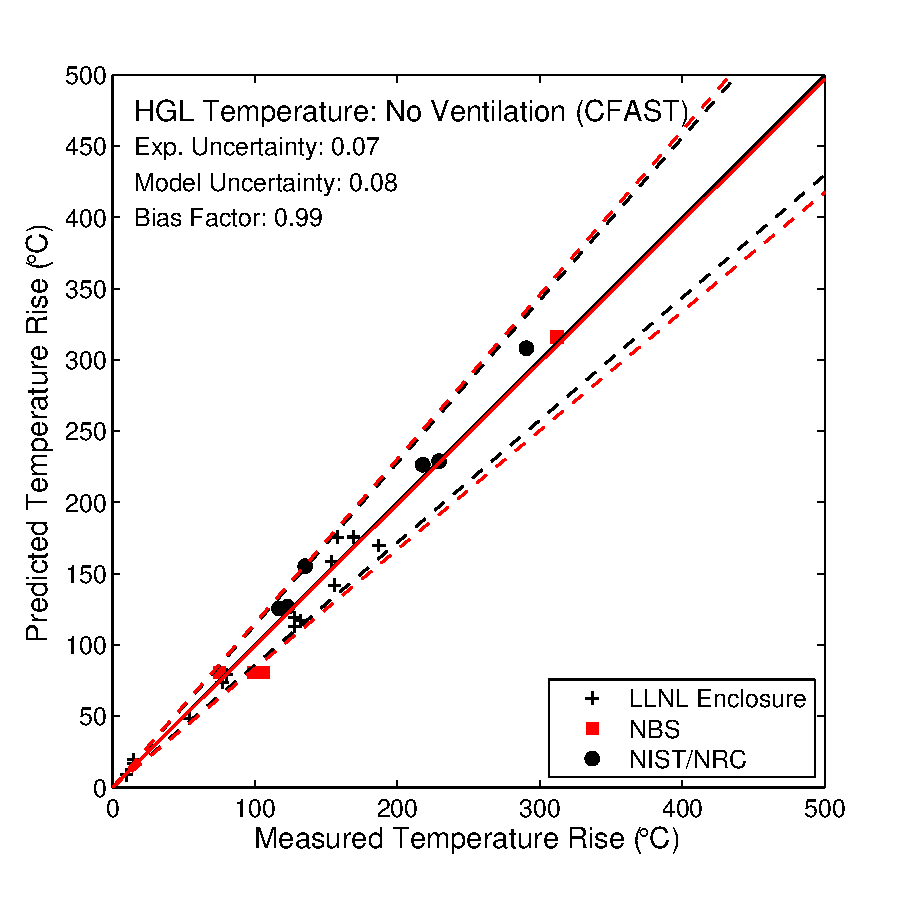
\includegraphics[width=3.0in]{FIGURES/ScatterPlots/HGL_Temperature_No_Ventilation}} \\
\end{tabular*}
\caption{Overall comparison of Measured and Predicted HGL Temperature.} \label{fig:HGL_Temperature_Scatter}
\end{figure}

\begin{figure}
\begin{tabular*}{\textwidth}{l@{\extracolsep{\fill}}r}
\multicolumn{2}{c}{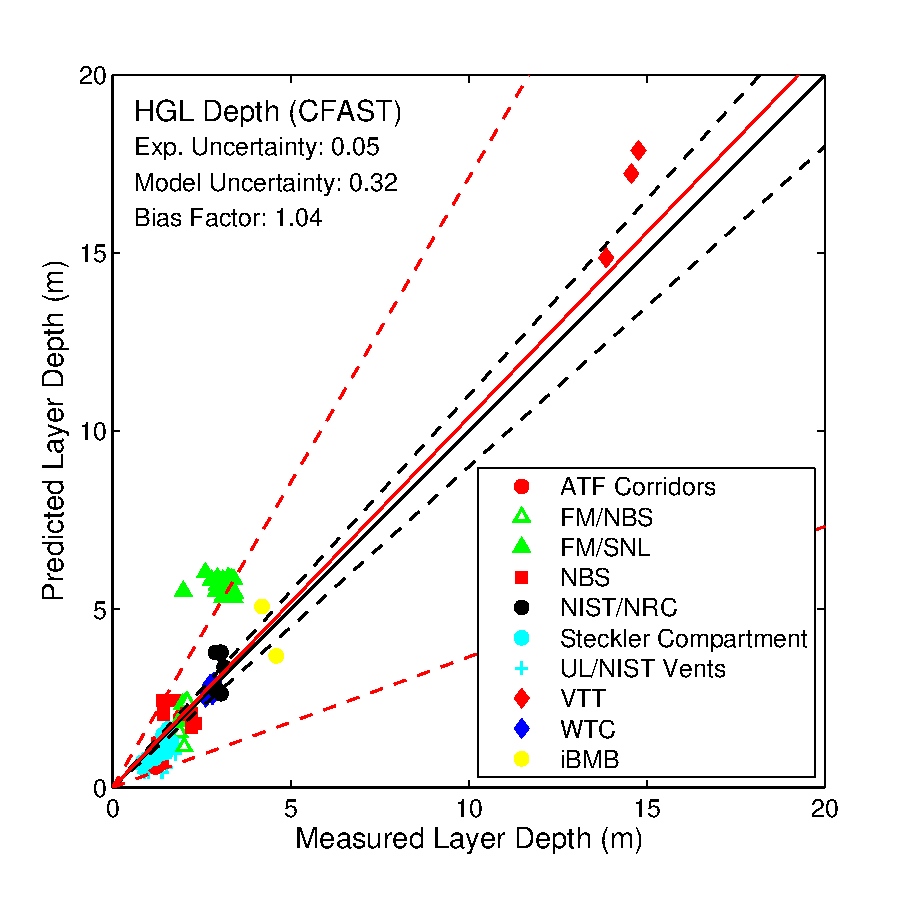
\includegraphics[width=3.0in]{FIGURES/ScatterPlots/HGL_Depth}} \\
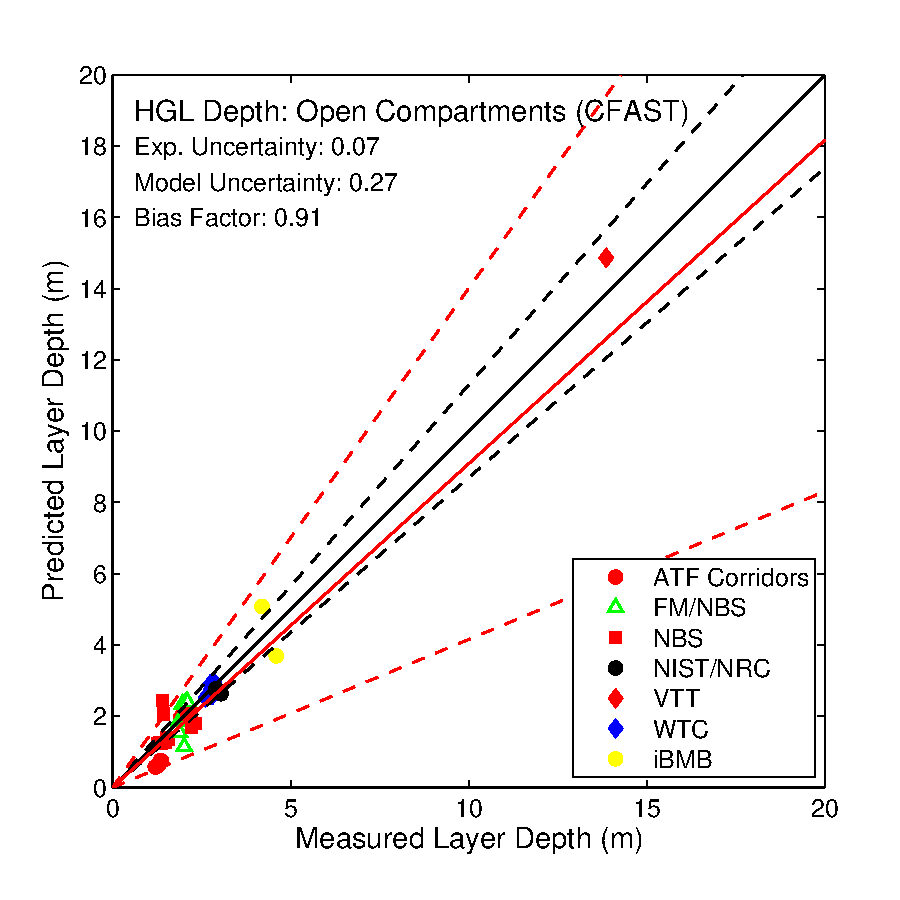
\includegraphics[width=3.0in]{FIGURES/ScatterPlots/HGL_Depth_Open_Compartments} &
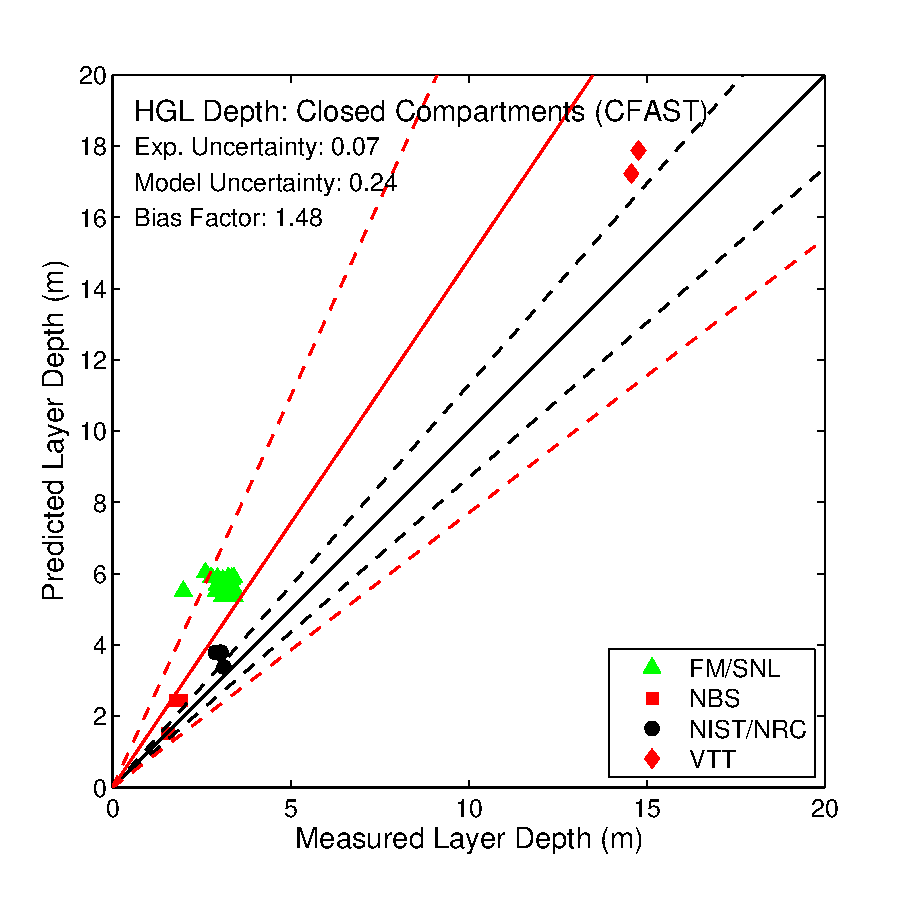
\includegraphics[width=3.0in]{FIGURES/ScatterPlots/HGL_Depth_Closed_Compartments}
\end{tabular*}
\caption{Overall comparison of Measured and Predicted HGL Height.} \label{fig:HGL_Height_Scatter}
\end{figure}

The two-zone assumption inherent in CFAST, modeled as a series of ordinary differential equations that describe mass and energy conservation of flows in a multiple-compartment structure typically provide prediction of gas layer temperature and layer height for the applications studied.

\begin{itemize}
\item The CFAST predictions of the HGL temperature and height are, with exceptions, are clustered near experimental uncertainty. On average, predicted HGL temperature is within \HGLtempavg~\% and HGL depth is within \HGLhgtavg~\% of experimental measurements. The CFAST predictions are typical of those found in other studies where the HGL temperature is typically somewhat over-predicted and HGL height somewhat lower (HGL depth somewhat thicker) than experimental measurements. These differences are likely attributable to simplifications in the model dealing with mixing between the layers, entrainment in the fire plume, and flow through vents.
\item Calculation of HGL temperature and height has higher uncertainty in rooms remote from the fire compared to those in the fire compartment.  Most likely, this is due to a combination of the simplified vent flow predictions (based on idealized Bernoulli flow) and the assumption of constant compartment surface thermal properties that are assumed independent of temperature.
\item It is worth noting that the UL/NIST Vents tests which include large vents in the ceiling of the test compartment show particularly higher HGL temperatures and corresponding smaller upper layer volume compared to experimental values.  Without these tests, the model uncertainties would be significantly lower.  This is likely due to the large size of the vents relative to those included in the original experimental correlations used by CFAST.
\end{itemize}




